\newpage
\section{Example: IndexOf}

To better illustrate verification in Whiley, we'll consider specifying a simple function.  This is the \lstinline{contains()} function, described as follows:

\begin{lstlisting}
// Return the lowest index in the items list which equals the given item.
// If no such index exists, return null.
function indexOf([int] items, int item) => int|null:
    ...
\end{lstlisting}

This is a common function found in the standard libraries of many
programming languages.  The body of the function examines each element
of the \lstinline{items} list and check whether or not it equals
\lstinline{item}.  To start with, we won't worry too much about the
body of the \lstinline{indexOf()} function.  Instead, we'll
progressively build up the specification until we are happy with it.
Then, we'll give an implementation of the function which meets this
specification.\\

\noindent To specify this function, we want to ensure three properties:

\begin{enumerate}
\item If the return is an integer \lstinline{i}, then
  \lstinline{items[i] == item}.
\item If the return is \lstinline{null}, there is no index
  \lstinline{j} where \lstinline{items[j] == item}.
\item If the return is an integer \lstinline{i}, then there is
  no index \lstinline{j} where \lstinline{j < i} and
  \lstinline{items[j] == item}.
\end{enumerate}

These properties determine how a correct implementation of the
\lstinline{indexOf()} function should behave.  We refer to them as the
{\em specification} of the \lstinline{indexOf()} function.

\subsection{Property 1 --- Return Valid Indexes}

The first of the above properties is the easiest, so lets start by
specifying that in Whiley.  At the same time, we'll also give an
initial implementation which satisfies this partial specification:

\begin{lstlisting}
function indexOf([int] items, int item) => (int|null r)
// If return value is an int i, then items[i] == item
ensures i is int ==> items[i] == item:
    //
    if |items| > 0 && items[0] == item:
        return 0
    else:
        return null
\end{lstlisting}

Here, we can see property (1) above written as an \lstinline{ensures}
clause in Whiley.  In particular, the phrase ``the return value is an
integer'' is translated into the condition ``\lstinline{i is int}''.
Likewise, the implication operator (i.e. \lstinline{==>}) is used to
say ``If ... then ...''.  We've also given an initial implementation
for the \lstinline{indexOf()} function which simply checks whether or
not \lstinline{items[0] == item}.  This implementation meets the
specification we have so far although, obviously, this is an
incomplete implementation of the \lstinline{indexOf} function!

\subsection{Property 2 --- Return Null if No Match}
Property (2) from our list above is more difficult to specify, because
it requires {\em quantification}.  There are several quantifiers
available in Whiley, including: \lstinline{all}, which allows us to
say ``for all elements in a list something is true''; and
\lstinline{no}, which allows us to say ``there is no element in the list
where something is true''. 

In Whiley, we can express property (2) from above in several different
ways.  The most direct translation would be:

\begin{lstlisting}
...
// If return is null, there is no index j where items[j] == item
ensures i is null ==> no { j in 0..|items| | items[j] == item }:
    ...
\end{lstlisting}

\noindent Here, the expression \lstinline{|items|} gives the length of
the items list, whilst the range expression \lstinline{0..|items|}
returns a list of consecutive integers from \lstinline{0} up to, but
not including, \lstinline{|items|}.  Instead of using the
\lstinline{no} quantifier, we could have equally used the
\lstinline{all} quantifier, like so:

\begin{lstlisting}
...
// If return is null, there is no index j where items[j] == item
ensures i is null ==> all { j in 0..|items| | items[j] != item }:
    ...
\end{lstlisting}

The above, however, is perhaps not as clear as the first translation.
Finally we can, in this case, avoid talking about indices altogether
like so:

\begin{lstlisting}
...
// If return is null, there is no index j where items[j] == item
ensures i is null ==> no { x in items | x == item }:
    ...
\end{lstlisting}

The above simple says ``there is no element \lstinline{x} in
\lstinline{items} where \lstinline{x == item}''.  Although this is
also not the most direct translation of the original property, it is a
rather convenient translation which achieves the same thing.

\subsection{Property 3 --- Return Least Index}
\subsection{Final Version}

At this point, we can now give the complete specification for the
\lstinline{indexOf()} function, along with an initial implementation:

\begin{lstlisting}
function indexOf([int] items, int item) => (int|null i)
// If return is an int r, then items[r] == item
ensures i is int ==> items[i] == item
// If return is null, then no element x in items where x == item
ensures i is null ==> no { x in items | x == item }
// If return is an int i, then no index j where j $<$ i and items[j] == item
ensures i is int ==> no { j in 0 .. i | items[j] == item }:
    //
    i = 0
    while i < |items|:
       if items[i] == item:
           return i 
       i = i + 1
    //
    return null
\end{lstlisting}

The implementation of \lstinline{indexOf()} given above meets the
function's specification.  Unfortunately, whilst this is true, the
Whiley compiler needs help to determine this.  Figure~\ref{eg_indexOf}
illustrates what happens when we compile the above code with
verification enabled.

\begin{figure}[!t]
\centering
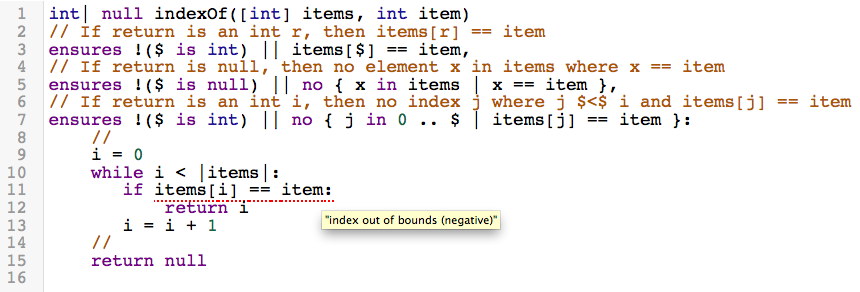
\includegraphics[width=1.0\textwidth]{../images/indexOf.png}
\caption{Illustrating our first working version of the
  \lstinline{indexOf} function being compiled with verification
  enabled.  The compiler is reporting an error stating ``{\em index out of
  bounds (negative)}''.  This is because the compiler believes
  \lstinline{i} may be negative at this point.  Although we know this
  is not true, we must write a {\em loop invariant} to help the
  compiler see this.}
\label{eg_indexOf}
\end{figure}
